% $Id: INF_Poster_example.tex 7714 2011-08-31 17:34:46Z tkren $
%
% TU Wien - Faculty of Informatics
% poster template
%
% This template is using the beamer document class and beamerposter package, see
% <http://www.ctan.org/tex-archive/macros/latex/contrib/beamer/>
% <http://www.ctan.org/tex-archive/macros/latex/contrib/beamerposter/>
% <http://www-i6.informatik.rwth-aachen.de/~dreuw/latexbeamerposter.php>
%
% For questions and comments send an email to
% Thomas Krennwallner <tkren@kr.tuwien.ac.at>
%

\documentclass[final,hyperref={pdfpagelabels=true}]{beamer}

\usepackage{TUINFPST}

\usepackage{lipsum}

\usepackage{graphicx}
\graphicspath{ {figures/} }

%\title[Computational Intelligence]{Interactive Computer Generated Architecture}
% if you have a long title looking squeezed on the poster, just force
% some distance:
\title[Communication and Media Engineering]{Distributed Flow Control and Intelligent Data Transfer in High Performance Networks}
% if you have a long title looking squeezed on the poster, just force
% some distance:
% \title[Computational Intelligence]{%
%   Integration of Conjunctive Queries over \\[0.2\baselineskip]%
%   Description Logics into HEX-Programs %\\[0.2\baselineskip]%
% }
\author[msadeghi@stud.hs-offenburg.de]{Mehdi Sadeghi}
\institute[]{%
  Hochschule für Technik, Wirtschaft und Medien Offenburg\\[0.25\baselineskip]
  Fakultät Medien und Informationswesen\\[0.25\baselineskip]
  %Arbeitsbereich: Wissensbasierte Systeme\\[0.25\baselineskip]
  Professorin: Dr. Katharina Mehner-Heindl\\[0.25\baselineskip]
  Betreuer: Dr. Adham Hashibon
}
%\institute{
%Fraunhofer Institute for Mechanics of Materials IWM\\[0.25\baselineskip]
%Wöhlerstraße 11\\[0.25\baselineskip]
%79108 Freiburg \\[0.25\baselineskip]
%Betreuer: Dr. Adham Hashibon}
\titlegraphic{\includegraphics[height=52mm]{iwm}}
\date[\today]{\today}
\subject{epilog}
\keywords{my kwd1, my kwd2}

%%%%%%%%%%%%%%%%%%%%%%%%%%%%%%%%%%%%%%%%%%%%%%%%%%%%%%%%%%%%%%%%%%%%%%%%%%%%%%%%%%%%%%

% Display a grid to help align images 
%\beamertemplategridbackground[12.7mm]

% play around with the background colors
% \setbeamercolor{background canvas}{bg=yellow}

% use a background picture
% \usebackgroundtemplate{%
%   \includegraphics[width=\paperwidth]{logo_KBS_2_CMYK}
% }

% play around with block colors
\setbeamercolor{block body}{fg=black,bg=white}
\setbeamercolor{block title}{fg=TuWienBlue,bg=white}

\setbeamertemplate{block begin}{
  \begin{beamercolorbox}{block title}%
    \begin{tikzpicture}%
      \node[draw,rectangle,line width=3pt,rounded corners=0pt,inner sep=0pt]{%
        \begin{minipage}[c][2cm]{\linewidth}
          \centering\textbf{\insertblocktitle}
        \end{minipage}
      };
    \end{tikzpicture}%
  \end{beamercolorbox}
  \vspace*{1cm}
  \begin{beamercolorbox}{block body}%
}

\setbeamertemplate{block end}{
  \end{beamercolorbox}
  \vspace{2cm}
}

% setup postit
\setbeamercolor{postit}{fg=black,bg=yellow} 
\newenvironment{postit}
{\begin{beamercolorbox}[sep=1em,wd=7cm]{postit}}
{\end{beamercolorbox}}


% for crop marks, uncomment the following line
\usepackage[cross,width=88truecm,height=123truecm,center]{crop}

%%%%%%%%%%%%%%%%%%%%%%%%%%%%%%%%%%%%%%%%%%%%%%%%%%%%%%%%%%%%%%%%%%%%%%%%%%%%%%%%%%%%%%

\begin{document}

% We have a single poster frame.
\begin{frame}
\fontsize{30pt}{31}\selectfont
  \begin{columns}[t]
    % ---------------------------------------------------------%
    % Set up a column
    \begin{column}{.45\textwidth}
      \begin{block}{Introduction}
Scientific experiments are the source of many high performance computing (HPC) problems. Here are
some highlights:

\begin{itemize}
\item Multiple simulation programs run during one operation
\item Huge data is being used by these programs
\item Data is being produced and used on the fly
\item Simplest form of workflow management is writing scripts
\item Users have to manage input/output files manually
\item Job schedulers have control over execution process
\end{itemize}

      This thesis is an effort to:% bring \textbf{control} and \textbf{ease of use} in above context:
      \begin{itemize}
      \item Accomplish operations on a distributed network collectively
      \item Make users neglectful of data location
      \item Propose a decentralized approach toward workflow management
      \item Avoid unnecessary data transfer
      \end{itemize}

      \end{block}
      
      \begin{block}{Requirements}
      The main points according to our context are these:
        \begin{itemize}
        \item \textbf{Data location is unknown} to users
        \item User should have same experience regardless of the peer to which she connects.
        \item System should have \textbf{no central brokers}.
        \item Required data are distributed on the network.
        \item \textbf{Runtime control} over task execution.
        \item The solution should be \textbf{distributed}.
        \item Easily deployable.
        \item \textbf{User space} solution
        \item Light weight
        \end{itemize}
      \end{block}

      \begin{block}{Related Work}
        There are similar solutions, some very localized and some too big for small groups to handle:
        \begin{itemize}
        \item UNICORE: a grid computing technology for resources such as supercomputers or cluster systems and information stored in databases.
        \item Distributed File Systems, centralized or decentralized
        \item Porto: The Porto platform will provide a lightweight and flexible system for data and workflow management.
        \end{itemize}
      \end{block}


      \begin{block}{Main Scenarios}
      We categorize every possible operation into two main groups:
      \begin{enumerate}
      \item \textbf{Linear}. These operations could be run in parallel. The algebraic notation would be:
      \[ Operation(A + B) = Operation(A) + Operation(B) \]
      \item \textbf{Non-linear}. These operations are different, they can't be run in parallel:
      \[ Operation(A + B) \neq Operation(A) + Operation(B) \]
      \end{enumerate}
      \end{block}

      \begin{block}{Proposed Solution}
      \textbf{We need only to solve two problems}:
      \begin{enumerate}
      \item How to solve an operation on one dataset?
      \item How to solve a non-linear operation on two datasets?
      \end{enumerate}
      \textbf{We break down all others into combinations of these two scenarios.}
      
      We propose to make a peer-to-peer collaborative application which will run on every resource 
      (computer) in our network, this computer (which we call it peer) will then become one part of 
      the network. In the beginning there is a network with any given number of peers,
      new ones can join and current ones can leave the network.
      
       Here are the main characteristics:
      \begin{itemize}
      \item The solution is \textbf{peer-to-peer}
      \item \textbf{Not a client/server} notion
      \item Based on \textbf{publish-subscribe} pattern
      \item Operations are \textbf{asynchronous}
      \item API calls return a \textbf{unique operation ID}
      \item Distributed operation store will be synchronized with peers
      \item \textbf{Peers subscribe to each other}
      \item Every \textbf{pear publishes news} on every \textbf{state changes}
      \item Peer can launch operations \textbf{recursively} on itself or others
%      \item Peers can launch operations on others
      \item Peers keep state for \textbf{Operations}, \textbf{Datasets} and other \textbf{peer list}
      \item Peers and application components are \textbf{loosely coupled}
      \end{itemize}
      
      In our design the simplest operation is not dependent on any other operation, and we know how to handle it. Other operations are made from these atomic ones.
      
      \end{block}
      
    \end{column}
    % ---------------------------------------------------------%
    % end the column

    % ---------------------------------------------------------%
    % Set up a column 
    \begin{column}{.45\textwidth}

      \begin{block}{A Sample Scenario}
      \begin{enumerate}
      \item User sends \(Op(A + B) \) to a \textbf{random} peer and gets an ID
      \item The peer stores this operation in a \textbf{distributed store}
      \item System breaks this to \(Op(A) + Op(B) \) and \textbf{self-launches} them \textbf{asynchronously}.
      \item Upon completion of sub-operations a random peer will store the result on the network and notify others
      \end{enumerate}
        %\alert{Watch out for } \cite{ff2010}
        Here is a demonstration of the interactions in sender and receiver peers:
 
               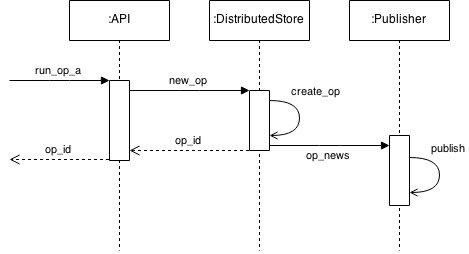
\includegraphics[]{kseq}             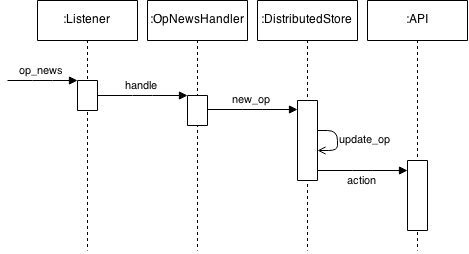
\includegraphics[]{kseq2}
      \end{block}
      
      \begin{block}{Internal Components}
      This figure demonstrates the main parts which form the internals of the application (and consequently each peer):\\
      
      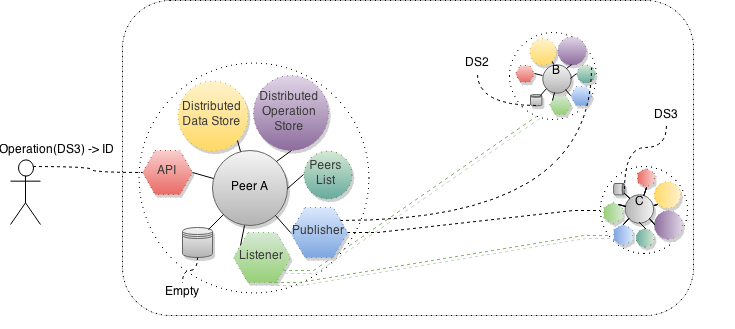
\includegraphics[width=\textwidth]{sys2}
      
      The above illustration shows:
      \begin{itemize}
      \item A network with three peers, labeled left to right as A, B and C respectively
      \item Publish/subscribe links between the peer in the left with the other two
      \item Local data store of each peer
      \item State objects of the peers including
      \begin{itemize}
      \item DistributedDataStore
      \item DistributedOperationStore
      \item Peers list
      \end{itemize}
      \item A basic submission scenario
      \item API, Publisher and Subscriber components
      \end{itemize}
      \end{block}
      
	  \begin{block}{Conclusion}
	  Even though there are many solutions designed for HPC problems, still there are requirements for smaller groups which are not satisfied, such as:
	  \begin{itemize}
	  \item Making scientific applications user friendly 
	  \item Providing \textit{smarter} solutions which get out of users way, i.e. hiding the systems complexity from ordinary users
	  \item The system manages data endpoints, not users
	  \item Less deployment and maintenance cost
	  \item More flexibility to control application at runtime
	  \end{itemize}
	  During this work we addressed some of these needs:
	  \begin{itemize}
	  \item The problem was defined and requirements where defined
	  \item We went through the state of the art
	  \item A solution approach was proposed
	  \item A prototype was developed
	  \begin{itemize}
	  \fontsize{30pt}{31}\selectfont
	  \item Based on open technologies
	  \item Runs in user space
	  \item Open source and freely available on Github
	  \end{itemize}
	  \end{itemize}
	  Our approach is very flexible to be extended and it is easy to build new services on top of the existing framework 
	  which provides the distributed operation and storage mechanisms to applications.
	  \end{block}
      \begin{block}{References}
      \fontsize{17pt}{18}\selectfont
        % this is just an example, use BibTeX!
        \begin{thebibliography}{999}
        \bibitem[UNICORE]{unicore}
        UNICORE article on Wikipedia
        \url{http://en.wikipedia.org/wiki/UNICORE}
        
        \bibitem[Porto]{porto}
        The Porto platform
        \url{https://github.com/NanoSim/Porto}
        
        \bibitem[konsensus]{konsensus}
        The Konsensus project \url{https://github.com/mehdisadeghi/konsensus}
%        \bibitem[Foo~and~Fu, 2010]{ff2010}
%          Foo, B.; and Fu, B.
%          2010.
%          \newblock {On logical representations of hackerisms}.
%          {\em J.~Log.~Hack.} 1:1--2.
%          
%        \bibitem[Crock~et~al., 2010]{ck2010}
%          Crock, A; Cruft, B.; and Kludge, C.
%          2010.
%          \newblock {Decomposing junk code}.
%          Manuscript.
          
        \end{thebibliography}
      \end{block}
    \end{column}
    % ---------------------------------------------------------%
    % end the column
  \end{columns}

%  \begin{tikzpicture}[remember picture,overlay]
%    \node[inner sep=0pt,xshift=-30cm,yshift=23cm] at (current page.east) {%
%      \begin{postit}%
%        Post-It time!%
%      \end{postit}%
%    }; 
%  \end{tikzpicture}
  
\end{frame}

\end{document}

%%% Local Variables:
%%% TeX-PDF-mode: t
%%% TeX-debug-bad-boxes: t
%%% TeX-master: t
%%% TeX-parse-self: t
%%% TeX-auto-save: t
%%% reftex-plug-into-AUCTeX: t
%%% End:
